\documentclass[a4paper,12pt]{article}

% --- Packages ---
\usepackage[utf8]{inputenc}
\usepackage[greek,english]{babel}
\usepackage{alphabeta}
\usepackage{amsmath,amssymb,amsfonts}
\usepackage{graphicx}
\usepackage{float}
\usepackage{geometry}
\usepackage{listings}
\usepackage{xcolor}
\usepackage{caption}
\usepackage{subcaption}
\usepackage{hyperref}
\usepackage{fancyhdr}

\geometry{margin=2.5cm}

% --- Code listing style ---
\lstdefinestyle{python}{
    language=Python,
    basicstyle=\ttfamily\small,
    keywordstyle=\color{blue}\bfseries,
    stringstyle=\color{red},
    commentstyle=\color{gray}\itshape,
    numbers=left,
    numberstyle=\tiny\color{gray},
    numbersep=8pt,
    frame=single,
    breaklines=true,
    breakatwhitespace=true,
    tabsize=4,
    showstringspaces=false,
    captionpos=b,
}

% --- Header/Footer ---
\pagestyle{fancy}
\fancyhf{}
\fancyhead[L]{Εργασία 2η -- Στοχαστικές Διεργασίες}
\fancyhead[R]{Βασία Βλάχου -- ΑΕΜ 6840}
\fancyfoot[C]{\thepage}

\begin{document}

% ============================
% TITLE PAGE
% ============================
\begin{titlepage}
    \centering
    \vspace*{2cm}

    {\LARGE \textbf{Εργασία 2η}}\\[0.5cm]
    {\Large Ανάλυση Στοχαστικών Διεργασιών}\\[0.3cm]
    {\Large Εκτίμηση Φάσματος Ισχύος}\\[2cm]

    {\large
    \textbf{Βασία Βλάχου}\\[0.3cm]
    ΑΕΜ: 6840\\[2cm]
    }

    \vfill
    {\large \today}
\end{titlepage}

% ============================
% TABLE OF CONTENTS
% ============================
\tableofcontents
\newpage

% ============================
% SECTION 1: INTRODUCTION
% ============================
\section{Εισαγωγή}

Στην παρούσα εργασία μελετάμε μια πραγματική διακριτή στοχαστική διεργασία που αποτελείται από άθροισμα συνημιτονοειδών σημάτων με τυχαίες φάσεις. Συγκεκριμένα, η διεργασία ορίζεται ως:

\begin{equation}
    X[k] = \sum_{i=1}^{6} \cos(\omega_i k + \varphi_i), \quad k = 0, 1, \dots, N-1
    \label{eq:signal}
\end{equation}

όπου $\omega_i = 2\pi\lambda_i$ είναι οι γωνιακές συχνότητες και $\varphi_i$ οι τυχαίες φάσεις.

\subsection{Παράμετροι της διεργασίας}

Οι συχνότητες $\lambda_i$ δίνονται ως εξής:

\begin{table}[H]
    \centering
    \begin{tabular}{|c|c|c|}
        \hline
        \textbf{Συχνότητα} & \textbf{Τιμή (Hz)} & \textbf{Σχέση} \\
        \hline
        $\lambda_1$ & 0.12 & -- \\
        $\lambda_2$ & 0.30 & -- \\
        $\lambda_3$ & 0.42 & $\lambda_3 = \lambda_1 + \lambda_2$ \\
        $\lambda_4$ & 0.19 & -- \\
        $\lambda_5$ & 0.17 & -- \\
        $\lambda_6$ & 0.36 & $\lambda_6 = \lambda_4 + \lambda_5$ \\
        \hline
    \end{tabular}
    \caption{Συχνότητες της διεργασίας $X[k]$.}
    \label{tab:frequencies}
\end{table}

Οι αντίστοιχες γωνιακές συχνότητες υπολογίζονται:
\begin{equation}
    \omega_i = 2\pi\lambda_i
\end{equation}

Οι φάσεις έχουν τις ακόλουθες ιδιότητες:
\begin{itemize}
    \item Οι $\varphi_1, \varphi_2, \varphi_4, \varphi_5$ είναι \textbf{ανεξάρτητες} τυχαίες μεταβλητές, ομοιόμορφα κατανεμημένες στο $[0, 2\pi]$.
    \item $\varphi_3 = \varphi_1 + \varphi_2$ (εξαρτημένη φάση).
    \item $\varphi_6 = \varphi_4 + \varphi_5$ (εξαρτημένη φάση).
\end{itemize}

Το μήκος δεδομένων είναι $N = 8192$.

\subsection{Σημασία των εξαρτημένων φάσεων}

Το γεγονός ότι $\varphi_3 = \varphi_1 + \varphi_2$ και $\varphi_6 = \varphi_4 + \varphi_5$ σημαίνει ότι οι τρίτη και έκτη αρμονική δεν είναι ανεξάρτητες από τις υπόλοιπες. Αυτό μοντελοποιεί φαινόμενα \textbf{τετραγωνικής σύζευξης φάσης} (quadratic phase coupling), τα οποία εμφανίζονται σε μη γραμμικά συστήματα. Συγκεκριμένα:
\begin{align}
    \lambda_3 &= \lambda_1 + \lambda_2 \quad \text{και} \quad \varphi_3 = \varphi_1 + \varphi_2 \\
    \lambda_6 &= \lambda_4 + \lambda_5 \quad \text{και} \quad \varphi_6 = \varphi_4 + \varphi_5
\end{align}

Αυτή η δομή θα είναι ανιχνεύσιμη μέσω ανάλυσης ανώτερης τάξης (bispectrum), αλλά στα πρώτα δύο ερωτήματα εστιάζουμε στην κατασκευή του σήματος και στην εκτίμηση του φάσματος ισχύος (δεύτερης τάξης).

% ============================
% SECTION 2: QUESTION 1
% ============================
\newpage
\section{Ερώτημα 1: Κατασκευή του $X[k]$}

\subsection{Θεωρητική ανάλυση}

Για την κατασκευή του σήματος $X[k]$ ακολουθούμε τα εξής βήματα:

\begin{enumerate}
    \item \textbf{Ορισμός συχνοτήτων:} Υπολογίζουμε τις γωνιακές συχνότητες $\omega_i = 2\pi\lambda_i$ για κάθε $i = 1, \dots, 6$.

    \item \textbf{Δημιουργία τυχαίων φάσεων:} Παράγουμε τέσσερις ανεξάρτητες τυχαίες μεταβλητές $\varphi_1, \varphi_2, \varphi_4, \varphi_5 \sim \mathcal{U}[0, 2\pi]$ και υπολογίζουμε τις εξαρτημένες φάσεις $\varphi_3$ και $\varphi_6$.

    \item \textbf{Υπολογισμός σήματος:} Για κάθε δείγμα $k = 0, 1, \dots, N-1$:
    \begin{equation}
        X[k] = \sum_{i=1}^{6} \cos(2\pi\lambda_i k + \varphi_i)
    \end{equation}
\end{enumerate}

Αναλυτικά, το σήμα αναπτύσσεται ως:
\begin{align}
    X[k] &= \cos(2\pi \cdot 0.12 \cdot k + \varphi_1) \nonumber \\
          &+ \cos(2\pi \cdot 0.30 \cdot k + \varphi_2) \nonumber \\
          &+ \cos(2\pi \cdot 0.42 \cdot k + \varphi_3) \nonumber \\
          &+ \cos(2\pi \cdot 0.19 \cdot k + \varphi_4) \nonumber \\
          &+ \cos(2\pi \cdot 0.17 \cdot k + \varphi_5) \nonumber \\
          &+ \cos(2\pi \cdot 0.36 \cdot k + \varphi_6)
    \label{eq:signal_expanded}
\end{align}

\subsection{Στατιστικές ιδιότητες}

Η μέση τιμή της διεργασίας είναι:
\begin{equation}
    E[X[k]] = \sum_{i=1}^{6} E[\cos(\omega_i k + \varphi_i)]
\end{equation}

Για τους όρους με ανεξάρτητες φάσεις ($i = 1, 2, 4, 5$), επειδή $\varphi_i \sim \mathcal{U}[0, 2\pi]$:
\begin{equation}
    E[\cos(\omega_i k + \varphi_i)] = \frac{1}{2\pi} \int_0^{2\pi} \cos(\omega_i k + \varphi) \, d\varphi = 0
\end{equation}

Για τον όρο $i = 3$, αν και η $\varphi_3 = \varphi_1 + \varphi_2$ δεν είναι ομοιόμορφη στο $[0, 2\pi]$, μπορούμε να δείξουμε ότι η μέση τιμή εξακολουθεί να είναι μηδέν (αντίστοιχα για $i = 6$). Άρα:
\begin{equation}
    E[X[k]] = 0, \quad \forall k
\end{equation}

\subsection{Υλοποίηση σε Python}

\begin{lstlisting}[style=python, caption={Κατασκευή του σήματος $X[k]$}]
import numpy as np
import matplotlib.pyplot as plt

# Parameters
N = 8192

# Frequencies (Hz)
lambda1, lambda2 = 0.12, 0.30
lambda4, lambda5 = 0.19, 0.17
lambda3 = lambda1 + lambda2  # 0.42
lambda6 = lambda4 + lambda5  # 0.36

# Angular frequencies
omega1 = 2 * np.pi * lambda1
omega2 = 2 * np.pi * lambda2
omega3 = 2 * np.pi * lambda3
omega4 = 2 * np.pi * lambda4
omega5 = 2 * np.pi * lambda5
omega6 = 2 * np.pi * lambda6

# Random phases - uniform on [0, 2*pi]
np.random.seed(42)
phi1 = np.random.uniform(0, 2 * np.pi)
phi2 = np.random.uniform(0, 2 * np.pi)
phi4 = np.random.uniform(0, 2 * np.pi)
phi5 = np.random.uniform(0, 2 * np.pi)
phi3 = phi1 + phi2  # dependent phase
phi6 = phi4 + phi5  # dependent phase

# Construct X[k]
k = np.arange(N)
X = (np.cos(omega1 * k + phi1)
   + np.cos(omega2 * k + phi2)
   + np.cos(omega3 * k + phi3)
   + np.cos(omega4 * k + phi4)
   + np.cos(omega5 * k + phi5)
   + np.cos(omega6 * k + phi6))
\end{lstlisting}

\subsection{Αποτελέσματα}

Στο Σχήμα~\ref{fig:signal} παρουσιάζεται η χρονοσειρά $X[k]$ για τα πρώτα 500 δείγματα. Παρατηρούμε ότι το σήμα ταλαντώνεται γύρω από το μηδέν, κάτι αναμενόμενο αφού $E[X[k]] = 0$. Η πολυπλοκότητα του σχήματος αντανακλά την υπέρθεση των έξι αρμονικών με διαφορετικές συχνότητες.

\begin{figure}[H]
    \centering
    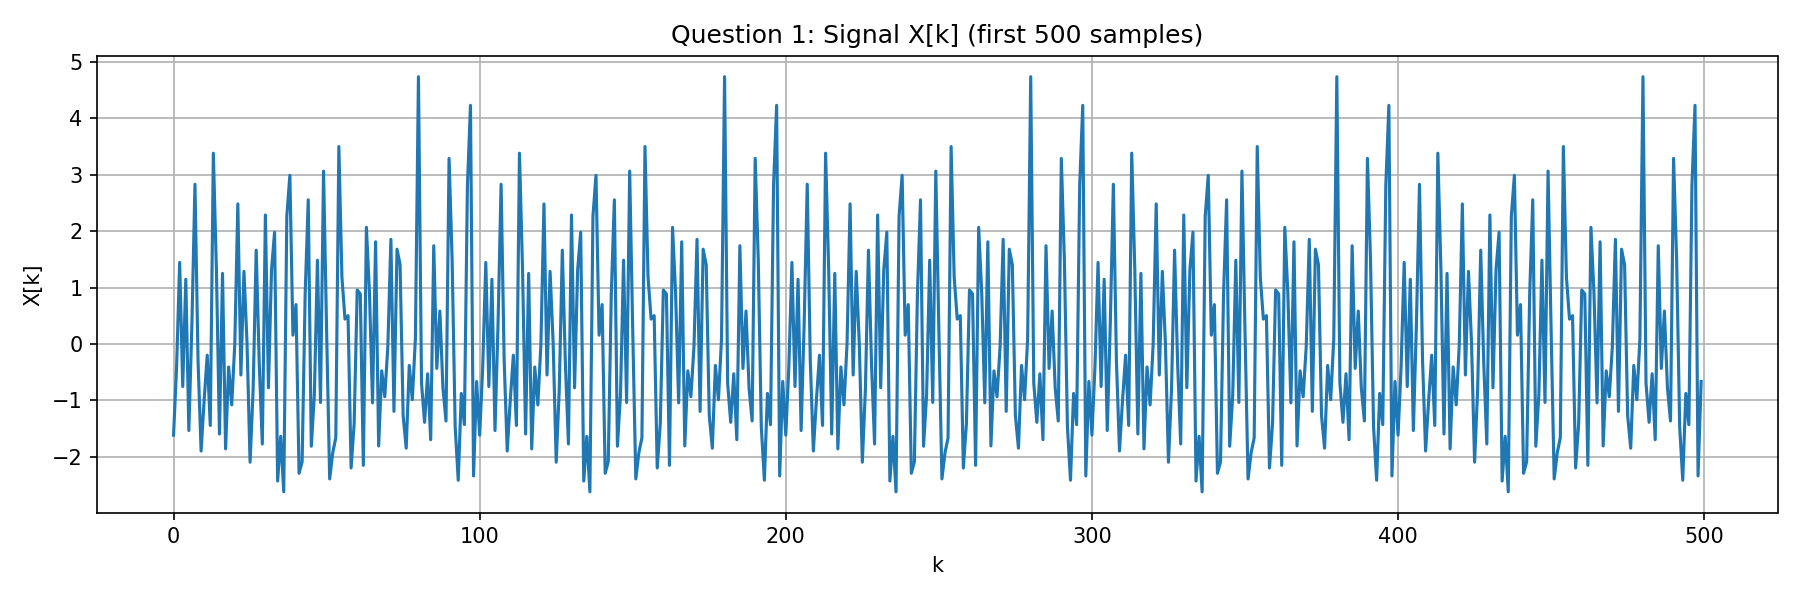
\includegraphics[width=\textwidth]{q1_signal.png}
    \caption{Χρονοσειρά $X[k]$ (πρώτα 500 δείγματα). Το σήμα αποτελεί υπέρθεση 6 συνημιτονοειδών αρμονικών με τυχαίες φάσεις.}
    \label{fig:signal}
\end{figure}

Το εύρος του σήματος κυμαίνεται περίπου στο $[-5, 5]$, κάτι λογικό αφού στη χειρότερη περίπτωση (όλα τα συνημίτονα σε φάση) θα είχαμε πλάτος $\pm 6$.

% ============================
% SECTION 3: QUESTION 2
% ============================
\newpage
\section{Ερώτημα 2: Εκτίμηση Φάσματος Ισχύος $C_x^*(f)$}

\subsection{Θεωρητική ανάλυση}

Η εκτίμηση του φάσματος ισχύος γίνεται μέσω της \textbf{μεθόδου αυτοσυσχέτισης} (Blackman-Tukey method). Η διαδικασία περιλαμβάνει δύο βήματα:

\subsubsection{Βήμα 1: Εκτίμηση αυτοσυσχέτισης}

Η εκτίμηση της συνάρτησης αυτοσυσχέτισης υπολογίζεται ως:
\begin{equation}
    \hat{R}_x[m] = \frac{1}{N} \sum_{k=0}^{N-1-|m|} X[k] \cdot X[k + |m|], \quad |m| \leq L_2
    \label{eq:autocorrelation}
\end{equation}

όπου $L_2 = 128$ είναι ο μέγιστος αριθμός ολισθήσεων. Η επιλογή $L_2 \ll N$ είναι σημαντική:
\begin{itemize}
    \item Μεγαλύτερο $L_2$: καλύτερη φασματική ανάλυση (στενότερες κορυφές) αλλά μεγαλύτερη διακύμανση.
    \item Μικρότερο $L_2$: χαμηλότερη διακύμανση αλλά χειρότερη φασματική ανάλυση (πλατύτερες κορυφές).
\end{itemize}

Στην περίπτωσή μας $L_2 = 128 \ll N = 8192$, που δίνει ένα καλό συμβιβασμό.

\subsubsection{Βήμα 2: Μετασχηματισμός Fourier της αυτοσυσχέτισης}

Το φάσμα ισχύος εκτιμάται ως ο μετασχηματισμός Fourier της αυτοσυσχέτισης:
\begin{equation}
    \hat{C}_x^*(f) = \sum_{m=-L_2}^{L_2} \hat{R}_x[m] \cdot e^{-j2\pi f m}
    \label{eq:power_spectrum}
\end{equation}

Επειδή η $\hat{R}_x[m]$ είναι πραγματική και άρτια συνάρτηση ($\hat{R}_x[m] = \hat{R}_x[-m]$), το φάσμα μπορεί να απλοποιηθεί:
\begin{equation}
    \hat{C}_x^*(f) = \hat{R}_x[0] + 2\sum_{m=1}^{L_2} \hat{R}_x[m] \cdot \cos(2\pi f m)
    \label{eq:power_spectrum_real}
\end{equation}

Αυτό εγγυάται ότι το εκτιμώμενο φάσμα είναι πραγματικό.

\subsection{Θεωρητικό φάσμα ισχύος}

Θεωρητικά, για μία στοχαστική διεργασία της μορφής $X[k] = \sum_i A_i \cos(\omega_i k + \varphi_i)$ με $A_i = 1$ και τυχαίες φάσεις, το φάσμα ισχύος αποτελείται από κορυφές Dirac στις συχνότητες $\lambda_i$:
\begin{equation}
    C_x(f) = \sum_{i=1}^{6} \frac{1}{2} \left[\delta(f - \lambda_i) + \delta(f + \lambda_i)\right]
\end{equation}

Κάθε συνημιτονοειδής όρος πλάτους 1 συνεισφέρει ισχύ $\frac{1}{2}$ σε κάθε μία από τις συχνότητες $\pm\lambda_i$. Η εκτίμηση $\hat{C}_x^*(f)$ θα πρέπει λοιπόν να εμφανίζει κορυφές στις 6 συχνότητες.

\subsection{Υλοποίηση σε Python}

\begin{lstlisting}[style=python, caption={Εκτίμηση φάσματος ισχύος μέσω αυτοσυσχέτισης}]
L2 = 128  # max shiftings

# Step 1: Estimate autocorrelation R_x[m]
lags = np.arange(-L2, L2 + 1)
Rx = np.zeros(len(lags))

for idx, m in enumerate(lags):
    m_abs = abs(m)
    Rx[idx] = (1.0 / N) * np.sum(X[:N - m_abs] * X[m_abs:N])

# Step 2: Power spectrum via DFT of autocorrelation
Nf = 1024  # frequency resolution points
f = np.linspace(0, 0.5, Nf)  # normalized frequency

Cx = np.zeros(Nf)
for i, fi in enumerate(f):
    Cx[i] = np.real(np.sum(
        Rx * np.exp(-1j * 2 * np.pi * fi * lags)
    ))
\end{lstlisting}

\subsection{Αποτελέσματα}

\begin{figure}[H]
    \centering
    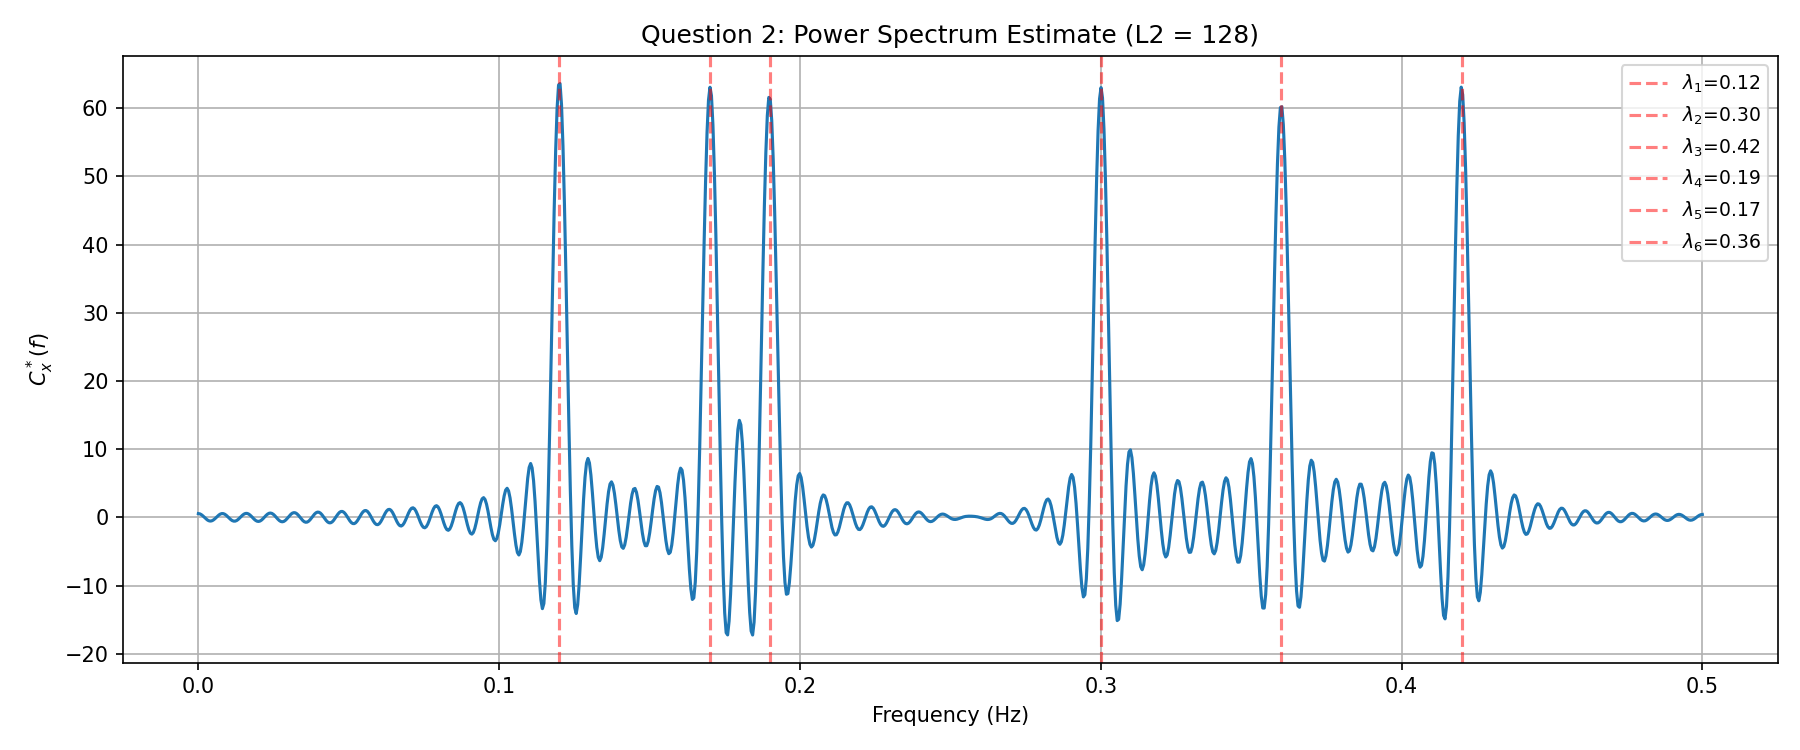
\includegraphics[width=\textwidth]{q2_power_spectrum.png}
    \caption{Εκτίμηση φάσματος ισχύος $\hat{C}_x^*(f)$ με $L_2 = 128$. Οι κόκκινες διακεκομμένες γραμμές υποδεικνύουν τις θεωρητικές συχνότητες $\lambda_i$.}
    \label{fig:spectrum}
\end{figure}

\subsubsection{Ανάλυση αποτελεσμάτων}

Από το Σχήμα~\ref{fig:spectrum} παρατηρούμε τα ακόλουθα:

\begin{enumerate}
    \item \textbf{Ταυτοποίηση κορυφών:} Εμφανίζονται ξεκάθαρα \textbf{6 κορυφές} στις αναμενόμενες συχνότητες:
    \begin{itemize}
        \item $\lambda_1 = 0.12$ Hz
        \item $\lambda_5 = 0.17$ Hz
        \item $\lambda_4 = 0.19$ Hz
        \item $\lambda_2 = 0.30$ Hz
        \item $\lambda_6 = 0.36$ Hz
        \item $\lambda_3 = 0.42$ Hz
    \end{itemize}

    \item \textbf{Ύψος κορυφών:} Όλες οι κορυφές έχουν παρόμοιο ύψος, κάτι αναμενόμενο αφού όλες οι αρμονικές συνεισφέρουν με πλάτος 1.

    \item \textbf{Πλάτος κορυφών:} Οι κορυφές δεν είναι ακριβώς κρουστικές (Dirac) αλλά έχουν πεπερασμένο πλάτος. Αυτό οφείλεται στο πεπερασμένο παράθυρο αυτοσυσχέτισης ($L_2 = 128$), το οποίο εισάγει ένα φαινόμενο \textbf{φασματικής διαρροής} (spectral leakage).

    \item \textbf{Πλευρικοί λοβοί:} Παρατηρούνται ταλαντώσεις (sidelobes) γύρω από κάθε κορυφή. Αυτές προκύπτουν από το ορθογώνιο παράθυρο που εφαρμόζεται σιωπηρά στην αυτοσυσχέτιση.

    \item \textbf{Διαχωρισμός κορυφών:} Οι κορυφές στα 0.17 Hz και 0.19 Hz βρίσκονται κοντά μεταξύ τους ($\Delta\lambda = 0.02$ Hz) αλλά διαχωρίζονται επαρκώς. Η φασματική ανάλυση (resolution) της μεθόδου είναι περίπου $\Delta f \approx 1/L_2 = 1/128 \approx 0.0078$ Hz, αρκετά μικρότερη από την απόσταση 0.02 Hz.
\end{enumerate}

\subsection{Φασματική ανάλυση (resolution)}

Η φασματική ανάλυση της μεθόδου Blackman-Tukey καθορίζεται από το $L_2$:
\begin{equation}
    \Delta f \approx \frac{1}{L_2} = \frac{1}{128} \approx 0.0078 \text{ Hz}
\end{equation}

Αυτό σημαίνει ότι μπορούμε να διαχωρίσουμε δύο κορυφές που απέχουν τουλάχιστον 0.0078 Hz. Στην περίπτωσή μας, η μικρότερη απόσταση μεταξύ κορυφών είναι $\lambda_4 - \lambda_5 = 0.19 - 0.17 = 0.02$ Hz $> \Delta f$, άρα ο διαχωρισμός είναι εφικτός.

% ============================
% SECTION 4: CONCLUSIONS
% ============================
\newpage
\section{Συμπεράσματα}

Στα δύο πρώτα ερωτήματα της εργασίας:

\begin{enumerate}
    \item \textbf{Κατασκευάσαμε} επιτυχώς τη στοχαστική διεργασία $X[k]$ ως υπέρθεση 6 συνημιτονοειδών αρμονικών με τυχαίες φάσεις. Η δομή εξάρτησης μεταξύ φάσεων ($\varphi_3 = \varphi_1 + \varphi_2$, $\varphi_6 = \varphi_4 + \varphi_5$) μοντελοποιεί τετραγωνική σύζευξη φάσης.

    \item \textbf{Εκτιμήσαμε} το φάσμα ισχύος $C_x^*(f)$ χρησιμοποιώντας τη μέθοδο αυτοσυσχέτισης (Blackman-Tukey) με $L_2 = 128$ μέγιστες ολισθήσεις. Το εκτιμώμενο φάσμα εμφανίζει ξεκάθαρα τις 6 αναμενόμενες κορυφές στις σωστές συχνότητες, επιβεβαιώνοντας την ορθότητα τόσο της κατασκευής του σήματος όσο και της μεθόδου εκτίμησης.
\end{enumerate}

Η μέθοδος αυτοσυσχέτισης παρέχει μια αξιόπιστη εκτίμηση δεύτερης τάξης του φάσματος, αλλά δεν μπορεί να ανιχνεύσει τις σχέσεις σύζευξης φάσης μεταξύ των αρμονικών -- αυτό απαιτεί ανάλυση ανώτερης τάξης (bispectrum), η οποία εξετάζεται σε επόμενα ερωτήματα.

\end{document}
